\documentclass[8pt, aspectratio=169]{beamer}
\usepackage[utf8]{inputenc}
\usepackage[magyar]{babel}
\usepackage{amsmath, amsfonts}
\usepackage{bm}
\usepackage{calc}
\usepackage{newtxmath}
\usepackage{microtype}
\usepackage{mathdots}
\usepackage{mathtools}
\usepackage{siunitx}

\usepackage{tikz}
\usetikzlibrary{shapes,arrows}
\usetikzlibrary{tikzmark,positioning}
\usepackage{pgfplots}
\usepgfplotslibrary{patchplots}
% 
% \definecolor{tkpblue}{rgb}{0.0, 0.627, 0.961}
% \definecolor{tkplightblue}{rgb}{0.455, 0.769, 0.937}
% \definecolor{tkplightgrey}{rgb}{0.851, 0.871, 0.910}
% \definecolor{tkpdarkgrey}{rgb}{0.3, 0.3, 0.35}     % for subtle lines or labels
% \definecolor{tkptext}{rgb}{0.294, 0.333, 0.392}
% \definecolor{tkphighlight}{rgb}{0.9, 0.5, 0.2}
% \definecolor{tkpgreen}{rgb}{0.2, 0.65, 0.35}    % fresh green
% \definecolor{tkpteal}{rgb}{0.0, 0.6, 0.6}       % balanced teal
% \definecolor{tkppurple}{rgb}{0.5, 0.3, 0.7}     % gentle violet
% \definecolor{tkpyellow}{rgb}{0.95, 0.75, 0.1}   % rich yellow
% \definecolor{tkplightyellow}{rgb}{1.0, 0.95, 0.75}
% \definecolor{tkpred}{rgb}{0.85, 0.2, 0.2}       % vivid red
% \definecolor{tkpbrown}{rgb}{0.6, 0.4, 0.2}      % earthy brown
% \definecolor{tkpmidgrey}{rgb}{0.6, 0.6, 0.7}       % for background reference

\definecolor{rd}{RGB}{178,34,34}
\definecolor{rd2}{RGB}{230,0,0}
\definecolor{gr}{RGB}{107,142,35}
\definecolor{gr2}{RGB}{0,209,0}
\definecolor{bl}{rgb}{0.0, 0.627, 0.961}
\definecolor{grey}{rgb}{0.651, 0.671, 0.710}
\definecolor{or}{RGB}{255,128,0}


% \pgfplotscreateplotcyclelist{tkpcolors}{
%   {color=tkpblue},
%   {color=tkpbrown},
%   {color=tkpred},
%   {color=tkpgreen},
%   {color=tkppurple},
%   {color=tkpteal}
% }
% 
% \pgfplotsset{
%   every axis/.append style={
%     cycle list name=tkpcolors
%   }
% }
% 
% \pgfplotsset{
%     colormap/tkpbluebrown/.style={
%         colormap={tkpbluebrown}{
%             rgb=(0.0, 0.627, 0.961)   % tkpblue
%             rgb=(0.9, 0.5, 0.2)      % tkphighlight (bridge color)
%             rgb=(0.6, 0.4, 0.2)      % tkpbrown
%         }
%     }
% }
% 
% 
% \pgfplotsset{
%     colormap/tkpbluegreen/.style={
%         colormap={tkpbluegreen}{
%             rgb=(0.0, 0.627, 0.961)    % tkpblue
%             rgb=(0.0, 0.6, 0.6)        % tkpteal
%             rgb=(0.2, 0.65, 0.35)      % tkpgreen
%             rgb=(0.95, 0.75, 0.1)      % tkpyellow
%             rgb=(0.9, 0.5, 0.2)        % tkphighlight
%         }
%     }
% }

\definecolor{PGreen}{HTML}{CDECCB}
\definecolor{POrange}{HTML}{FFE2C2}
\definecolor{PBlue}{HTML}{5E8CCB}
\definecolor{Charcoal}{HTML}{1F1F1F}

% Extra complementary colors:
\definecolor{PLightBrown}{HTML}{D6BFA3}  
\definecolor{PMedBrown}{HTML}{A67855}  
\definecolor{PDarkBrown}{HTML}{4B2E1E}

\definecolor{PLightBlue}{HTML}{B8D9EB}% light sky blue
\definecolor{PLightGray}{HTML}{E6E6E6} % for subtle backgrounds
\definecolor{PPurple}{HTML}{C4B4D9}     % muted pastel purple
\definecolor{PYellow}{HTML}{F9EBA5}     % slightly darker pastel yellow
\definecolor{PMauve}{HTML}{BFA1C8}  % pasztell lila
\usetheme[progressbar=none, numbering=fraction, titleformat=smallcaps]{metropolis}           % Use metropolis theme
\setbeamercolor{progress bar}{fg=PBlue}
\setbeamercolor{progress bar in head/foot}{fg=PBlue}
\setbeamercolor{progress bar in section page}{fg=PBlue}




\setbeamercolor{normal text}{fg=Charcoal,bg=white}
\setbeamercolor{structure}{fg=PBlue}

% Headline & titles
\setbeamercolor{title}{fg=PBlue!60!black}
\setbeamercolor{frametitle}{fg=white,bg=PBlue}
\setbeamercolor{titlelike}{fg=PBlue!60!black}
\setbeamercolor{title separator}{fg=PBlue}

% Blocks
\setbeamercolor{block title}{fg=Charcoal,bg=PLightGray!80}
\setbeamercolor{block body}{fg=Charcoal,bg=PLightGray!30}

\setbeamercolor{alerted text}{fg=POrange!70!red}

\setbeamercolor{block title alerted}{fg=Charcoal,bg=POrange}
\setbeamercolor{block body alerted}{fg=Charcoal,bg=POrange!50}
% 

% ---------- Section-szerinti számláló ----------
\newcounter{thm}[section]
\renewcommand{\thethm}{\thesection.\arabic{thm}}

% ---------- Saját theorem környezet ----------
\newenvironment{blockthm}[1][]{%
  \refstepcounter{thm}%
  \setbeamercolor{block title}{fg=Charcoal,bg=PLightBlue!80}%
  \setbeamercolor{block body}{fg=Charcoal,bg=PLightBlue!30}%
  \begin{block}{\thethm. Tétel#1}%
}{%
  \end{block}%
}

% ---------- Saját definition környezet ----------
\newenvironment{blockdef}[1][]{%
  \refstepcounter{thm}%
  \setbeamercolor{block title}{fg=Charcoal,bg=PYellow!80}%
  \setbeamercolor{block body}{fg=Charcoal,bg=PYellow!30}%
  \begin{block}{\thethm. Definíció#1}%
}{%
  \end{block}%
}

% ---------- Saját lemma környezet ----------
\newenvironment{blocklem}[1][]{%
  \refstepcounter{thm}%
  \setbeamercolor{block title}{fg=Charcoal,bg=PPurple!80}%
  \setbeamercolor{block body}{fg=Charcoal,bg=PPurple!30}%
  \begin{block}{\thethm. Lemma#1}%
}{%
  \end{block}%
}


% ---------- Saját lemma környezet ----------
\newenvironment{exercise}[1][]{%
  \refstepcounter{thm}%
  \setbeamercolor{block title}{fg=Charcoal,bg=PGreen!80}%
  \setbeamercolor{block body}{fg=Charcoal,bg=PGreen!30}%
  \begin{block}{\thethm. Feladat#1}%
}{%
  \end{block}%
}

\newcommand{\R}{\mathbb{R}}
\newcommand{\Z}{\mathbf{Z}}
\DeclareMathOperator*{\argmin}{arg\,min}
\DeclareMathOperator{\diag}{diag}
\DeclareMathOperator{\sat}{sat}
\DeclareMathOperator{\var}{Var}

\DeclareMathOperator{\dom}{dom}

\newcommand{\bx}{\mathbf{x}}
\newcommand{\ba}{\mathbf{a}}
\newcommand{\bhx}{\mathbf{\hat{x}}}
\newcommand{\by}{\mathbf{y}}
\newcommand{\bhy}{\mathbf{\hat{y}}}
\newcommand{\bu}{\mathbf{u}}
\newcommand{\bb}{\mathbf{b}}
\newcommand{\bF}{\mathbf{F}}
\newcommand{\bp}{\mathbf{p}}
\newcommand{\bd}{\mathbf{d}}
\newcommand{\bq}{\mathbf{q}}


\newcommand{\bA}{\mathbf{A}}
\newcommand{\bC}{\mathbf{C}}
\newcommand{\bX}{\mathbf{X}}
\newcommand{\bM}{\mathbf{M}}
\newcommand{\bH}{\mathbf{H}}
\newcommand{\bS}{\mathbf{S}}
\newcommand{\bI}{\mathbf{I}}
\newcommand{\bR}{\mathbf{R}}
\newcommand{\bQ}{\mathbf{Q}}


\newcommand{\bbeta}{\boldsymbol{\beta}}
\newcommand{\beps}{\boldsymbol{\epsilon}}
\newcommand{\bnu}{\boldsymbol{\nu}}
\newcommand{\blambda}{\boldsymbol{\lambda}}
\newcommand{\bSigma}{\boldsymbol{\Sigma}}


% % \renewtheorem{theorem}{Tétel}[section]
% \newtheorem{lemma}[theorem]{Lemma}
% \newtheorem{definition}[theorem]{Definíció}


\newcommand{\hl}[2][hlyellow]{\mathchoice%
 {\colorbox{#1}{$\displaystyle#2$}}%
 {\colorbox{#1}{$\textstyle#2$}}%
 {\colorbox{#1}{$\scriptstyle#2$}}%
 {\colorbox{#1}{$\scriptscriptstyle#2$}}}%


% \usefonttheme[onlymath]{serif}
\usepackage[sfdefault, lining]{FiraSans}
\renewcommand*\oldstylenums[1]{{\firaoldstyle #1}}


\renewcommand{\emph}[1]{{\bf #1}}


\newcommand{\nb}[2]{(#1)_{#2}}
\newcommand{\D}{\mathbb{D}}
\newcommand{\N}{\mathbb{N}}



\title{A Gausz-függvény univerzalitása}
\date{\today}
\author{Csikja Rudolf}

\begin{document}
\begin{frame}{}
\titlepage
\end{frame}

\begin{frame}{}
\tableofcontents
\end{frame}


\section{Bevezetés}
\begin{frame}[t]{A harang görbe jelentősége}
\begin{columns}
\begin{column}{0.4\textwidth}
\begin{center}
\includegraphics[scale=0.08]{Carl_Friedrich_Gauss_1840.jpg}\\
\textbf{Carl Friedrich Gauss} \\ (1777--1855) 
\end{center}
\end{column}

\begin{column}{0.6\textwidth}
Johann Carl Friedrich Gauss német matematikus, természettudós, csillagász.
\vspace{0.3cm}
\begin{itemize}
    \item \textit{„Princeps Mathematicorum”} – a matematikusok fejedelme.
    \item Már gyerekként (7 évesen) elkápráztatta tanárait a számok gyors összeadásával (1-től 100-ig).
    \item Alapvető műve a \textit{Disquisitiones Arithmeticae}, de maradandót alkotott a mágnességtanban (Gauss-törvény) és a földmérésben is.
    \item A statisztika alapjait a Ceres törpebolygó pályájának újrafelfedezésekor fektette le.
\end{itemize}
\end{column}
\end{columns}
\end{frame}

\begin{frame}{Miért éppen a haranggörbe?}
    A Gauss-függvény a természet „alapértelmezett” állapota.
    \begin{itemize}
        \item \textbf{Mérési hibák:} A véletlen hibák összeadódása természetes módon ezt a formát ölti.
        \item \textbf{Statisztikai stabilitás:} A centrális határeloszlástétel értelmében független hatások összege Gauss-eloszláshoz tart.
        \item \textbf{Fizikai invariancia:} 
        \begin{itemize}
            \item \textbf{Diffúzió és hővezetés:} A hővezetési egyenlet alapvető megoldása. Egy pontszerű forrásból induló hő vagy anyag eloszlása az időben mindig Gauss-görbe marad (csak ellaposodik).
            \item \textbf{Fourier-invariancia:} Az egyetlen függvénycsalád, amelynek Fourier-transzformáltja önmaga (szintén Gauss-függvény).
            \item \textbf{Entrópia-maximum:} Rögzített szórás mellett ez az eloszlás rendelkezik a legnagyobb entrópiával (a „legvéletlenebb” állapot).
        \end{itemize}
    \end{itemize}
\end{frame}

\begin{frame}{A 10 német márkás bankjegy (1991-–2001)}
    \begin{columns}
        \begin{column}{0.5\textwidth}
            Ritka megtiszteltetés a matematikában: a német állam Gauss portréja mellett magát a függvényt és annak képletét is a nemzeti fizetőeszközre nyomtatta.
            \vspace{0.5cm}
            \begin{itemize}
                \item Látható a standard Gauss-görbe.
                \item Mellette a sűrűségfüggvény képlete.
            \end{itemize}
        \end{column}
        \begin{column}{0.5\textwidth}
            \begin{center}
                % Itt hivatkozhatsz egy képre a bankjegyről
                \includegraphics[width=\textwidth]{./pictures/10_DM_bill.jpg} \\
                \footnotesize{A Gauss-görbe mint kulturális örökség.}
            \end{center}
        \end{column}
    \end{columns}
\end{frame}

\begin{frame}{}
    \begin{columns}
        \begin{column}[t]{0.5\textwidth}
            \begin{center}
                \includegraphics[width=0.6\textwidth]{./pictures/gauss_stamp_1955.jpg} \\
                \footnotesize{1955-ös NSZK bélyeg:\\ Halálának 100. évfordulójára.}
            \end{center}
        \end{column}
        \begin{column}[t]{0.5\textwidth}
            \begin{center}
                \includegraphics[width=0.7\textwidth]{./pictures/gauss_coin_1977.png} \\
                \footnotesize{1977-es érme:\\ Születsének 200. évfordulójára.}
            \end{center}
        \end{column}
    \end{columns}
\end{frame}


\section{A Gauss függvény elemi vizsgálata}

\subsection{Alapvető tulajdonságok}
\begin{frame}{A Standard Gauss-függvény}
 \begin{columns}
\begin{column}[t]{0.4\textwidth}
\begin{blockdef}[~ (Gauss függvény)]
A valós $g\colon \R \to \R$ függvényt
\[g(x) := \exp\left(-\frac{x^2}{2}\right)\]
(standard) Gauss függvénynek hívjuk.
\end{blockdef}
\begin{center}
  \pgfplotsset{width=\columnwidth,compat=1.9}
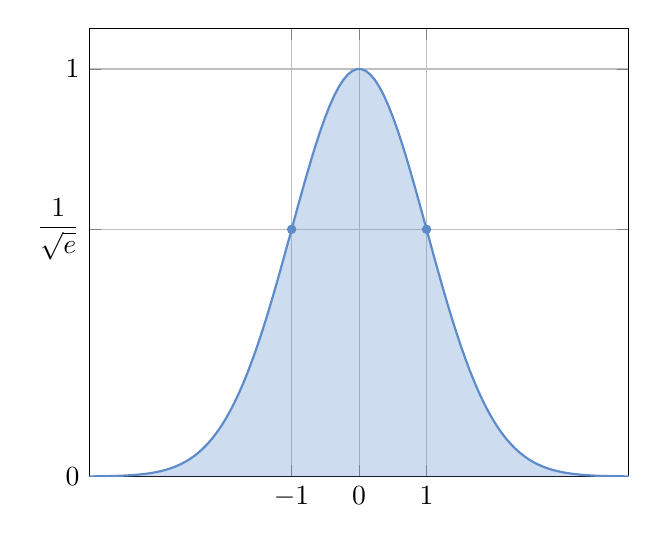
\begin{tikzpicture}[scale=1]
    \begin{axis}[
        xmin = -4, xmax = 4,
        ymin = -0.0, ymax = 1.1,
        mark=none,
        xtick={-1,0,1},
        ytick={0,{1/sqrt(e)}, 1},
        xticklabels={$-1$,$0$,$1$},
        yticklabels={$0$,$\dfrac{1}{\sqrt e}$,$1$},
        grid=major,
        minor tick num=0,
    ]
    \addplot[color=PBlue, fill=PBlue, fill opacity=0.3, domain=-5:5, thick, samples=150]{exp(-(x^2/2))};
    \addplot[
        only marks,
        mark=*,
        mark size=1.5pt,
        color=PBlue] 
            coordinates {
            (-1,{1/sqrt(e)})
            (1,{1/sqrt(e)})
            };
    \end{axis}
    
\end{tikzpicture}

\end{center}
\end{column}
\begin{column}[t]{0.6\textwidth}
\begin{block}{Elemi tulajdonságok}
\begin{enumerate}[a)]
 \item Pozitív $g(x)>0$ és páros $g(x) = g(-x)$.
 \item Sima függvény: $g\in C^\infty$.
 \item Globális maximuma van az $x=0$ pontban: $g(x)\le g(0)$, $x\in\R\setminus\{0\}.$
 \item Monoton növekvő a $(-\infty, 0),$ illetve monoton csökkenő a $(0, +\infty)$ intervallumon.
 \item Inflexiós pontja van az $x=1$ és $x=-1$ pontokban, továbbá konkáv a $(-\infty, -1)$ és az $(1, +\infty)$ intervallumokon, illetve konvex a $(-1, 1)$ intervallumon.
\end{enumerate}
\end{block}
\end{column}
\end{columns}
\end{frame}

\begin{frame}[t]{A Gauss-függvények családja}
Minden nem standard Gauss függvény megkapható a standard változat eltolásával és skálázásával,
pontosabban:
\[G_{\mu,\sigma}(x) := g\left(\frac{x-\mu}{\sigma}\right) = \exp\left(-\frac{(x-\mu)^2}{2\sigma^2}\right).\]
\vskip-0.8em
\begin{columns}
\begin{column}[t]{0.45\textwidth}
\begin{center}
  \pgfplotsset{width=0.5\columnwidth,compat=1.9}
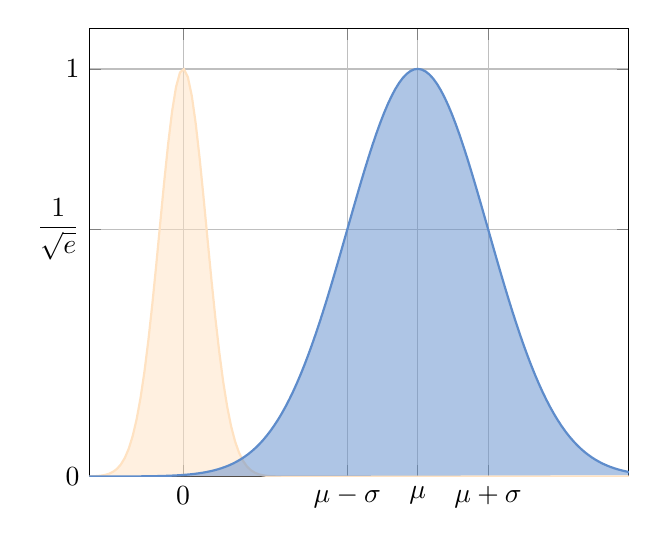
\begin{tikzpicture}[scale=1]
    \begin{axis}[
        xmin = -4, xmax = 19,
        ymin = -0.0, ymax = 1.1,
        mark=none,
        xtick={0,7,10,13},
        ytick={0,{1/sqrt(e)}, 1},
        xticklabels={$0$,$\mu-\sigma$, $\mu$, $\mu+\sigma$},
        yticklabels={$0$,$\dfrac{1}{\sqrt e}$,$1$},
        grid=major,
        minor tick num=0,
    ]
    \addplot[color=POrange, fill=POrange, fill opacity=0.5, domain=-5:20, thick, samples=150]{exp(-(x^2/2))};
    \addplot[color=PBlue, fill=PBlue, fill opacity=0.5, domain=-4:20, thick, samples=150]{exp(-((x-10)^2/(2*3^2))};
\end{axis}
\end{tikzpicture}

\end{center}
\end{column}
\begin{column}[t]{0.55\textwidth}
\begin{exercise}
Határozzuk meg azt az 
\[y'(x) = f(x, y(x))\]
alakú differenciálegyenletet, amelynek megoldása a standard Gauss-függvény.
\end{exercise}
\end{column}
\end{columns}
\end{frame}


\begin{frame}[t]{A cos függvény hatványai}
\begin{columns}
\begin{column}{0.4\textwidth}
\[f_n(x):=\cos^n(x), \quad x\in(-\pi/2, \pi/2)\] 
\begin{center}
\pgfplotsset{width=\columnwidth,compat=1.9}
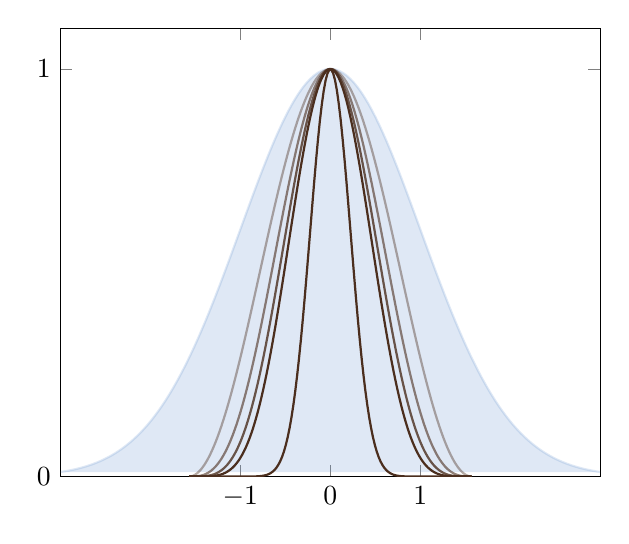
\begin{tikzpicture}[scale=1]
    \begin{axis}[
        trig format plots=rad,
        xmin = -3, xmax = 3,
        ymin = -0.0, ymax = 1.1,
        mark=none,
        xtick={-1,0,1},
        ytick={0, 1},
        xticklabels={$-1$,$0$,$1$},
        yticklabels={$0$,$1$}
    ]
    \addplot[color=PBlue, fill=PBlue, opacity=0.2, domain=-3:3, thick, samples=150]{exp(-(x^2/2))};
    \addplot[color=PDarkBrown, opacity=0.4, domain=-1.57:1.57, thick, samples=150]{cos(x)^2};
    \addplot[color=PDarkBrown, opacity=0.6, domain=-1.57:1.57, thick, samples=150]{cos(x)^3};
    \addplot[color=PDarkBrown, opacity=0.8, domain=-1.57:1.57, thick, samples=150]{cos(x)^4};
    \addplot[color=PDarkBrown, opacity=1.0, domain=-1.57:1.57, thick, samples=150]{cos(x)^5};
    \addplot[color=PDarkBrown, opacity=1.0, domain=-1.57:1.57, thick, samples=150]{cos(x)^20};

    \end{axis}
    
\end{tikzpicture}

\end{center}
\[\lim_{n\to\infty}f_n(s_n) = \frac{1}{\sqrt{e}}.\]
\end{column}
\begin{column}{0.6\textwidth}
A probléma, hogy az inflexiós pontok a nullához tartanak, és így a függvények egyre elvékonyodnak.
Sőt, az $f_n(x)$ értékek az origón kívül mindenhol nullához tartanak. 
Viszont, ha minden egyes függvénynek az inflexiós pontját az $x=1$
pontba transzformáljuk, akkor az így kapott új függvény-sorozat nem vékonyodik el.
Ezt úgy érhetjük el, hogy minden egyes függvényre átskálázzuk az értelmezési tartományt:
\[g_n(x):=f_n(s_n x) = \cos^n(s_n x), \quad  -\frac{\pi}{2s_n} \le x \le \frac{\pi}{2s_n}.\]
\end{column}
\end{columns}
\end{frame}

\subsection{Maximummal rendelkező függvények magas hatványai}
\begin{frame}[t]{Lokális koordináta}
\begin{columns}
  \begin{column}{0.4\textwidth}
    Az $f_n$ függvény $s_n>0$ inflexiós pontja
    \[\hl{s_n = \arctan\left(\frac{1}{\sqrt{n-1}}\right)}\]
  Az átskálázott $g_n$ függvény
  \[\hl{g_n(x) = \cos^n \left( \arctan\left(\frac{1}{\sqrt{n-1}}\right) x\right)}\]
  Az $g_n$ függvények értelmezési tartománya egyre nő:
\[\dom(g_n) = (-\pi/(2s_n), \pi/(2s_n)) \sim (-\pi \sqrt{n}, \pi \sqrt{n}).\]
  \end{column}
  \begin{column}{0.6\textwidth}
    \begin{center}
        \pgfplotsset{width=0.5\columnwidth,compat=1.9}
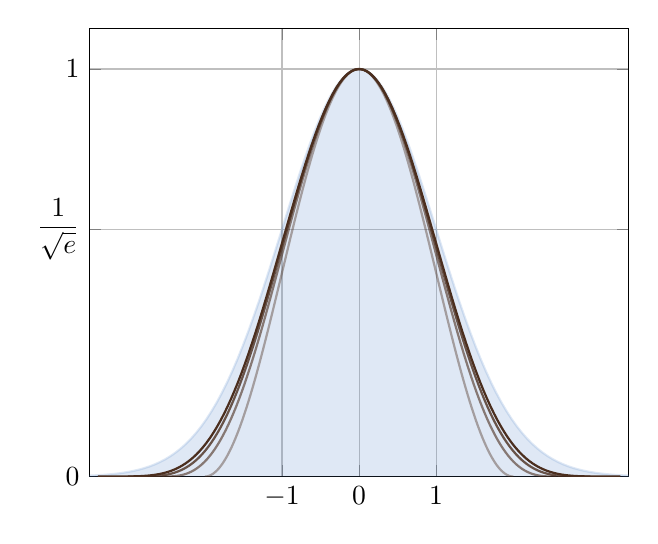
\begin{tikzpicture}[scale=1]
    \begin{axis}[
        xmin = -3.5, xmax = 3.5,
        ymin = -0.0, ymax = 1.1,
        mark=none,
        xtick={-1,0,1},
        ytick={0,{1/sqrt(e)}, 1},
        xticklabels={$-1$,$0$,$1$},
        yticklabels={$0$,$\dfrac{1}{\sqrt e}$,$1$},
        grid=major,
        minor tick num=0,
    ]
    \addplot[color=PBlue, fill=PBlue, opacity=0.2, domain=-5:5, thick, samples=150]{exp(-(x^2/2))};
    \addplot[color=PDarkBrown, opacity=0.4, domain=-2:2, thick, samples=150]{cos(x * 45)^2};
    \addplot[color=PDarkBrown, opacity=0.6, domain=-2.553:2.553, thick, samples=150]{cos(x * atan(1/sqrt(2)))^3};
    \addplot[color=PDarkBrown, opacity=0.8, domain=-3:3, thick, samples=150]{cos(x * 30)^4};
    \addplot[color=PDarkBrown, opacity=1.0, domain=-3.389:3.389, thick, samples=150]{cos(x * atan(0.5))^5};
    \end{axis}
    
\end{tikzpicture}

    \end{center}
  \end{column}
\end{columns}
Végtelen sok féle skálázás létezik, az általáunk választott az inflexiós pontokat egy pontba transzformálta, ennek nem kell így lennie,de aszimptotikusan meg kell, hogy egyezzenek:
\[s_n \sim \frac{1}{\sqrt{n}}\]
\end{frame}

\begin{frame}[t]{Konvergencia a Gauss-függvényhez}
A $g_n$ függvények ábrája azt sejteti, hogy a standard Gauss-függvényhez tartanak.
Erről meggyőződhetünk, ha a bonyolult szögfüggvényeket egyszerű polinomokkal közelítjük, amikor
$x\approx 0$ és $n\to\infty$. A közelítést alkalmazva:
\[g_n(x) \approx \cos^n \left(\frac{x}{\sqrt{n}}\right) \approx \left(1 - \frac{1}{2}\left(\frac{x}{\sqrt{n}}\right)^2\right)^n = \left(1 - \frac{x^2}{2n}\right)^n,\]
ami határértékben
\[\hl{\lim_{n\to\infty} g_n(x) = \lim_{n\to\infty}\left(1 - \frac{x^2}{2n}\right)^n = \exp\left(-\frac{x^2}{2}\right).}\]
\end{frame}

\begin{frame}[t]{Feladatok}
 \begin{columns}
  \begin{column}[t]{0.5\textwidth}
     \begin{exercise}
    Határozzuk meg az $f_n$ függvény $s_n > 0$ inflexiós pontját a $f_n''(s_n) = 0$ egyenlet megoldásával!
    \end{exercise}
    \begin{exercise}
    Bizonyítsuk be, hogy
    \begin{itemize}
     \item $g_n''(1) = 0$
     \item $\lim_{n\to\infty}g_n(1) = 1/\sqrt{e}$
     \item $\lim_{n\to\infty} \dom(g_n) = (-\infty, +\infty)$
    \end{itemize}
    \end{exercise}
  \end{column}
  
  \begin{column}[t]{0.5\textwidth}
    \begin{exercise}
     Ismételjük meg az eddigi számításokat az
     \begin{enumerate}[a)]
      \item $f_n(x):=\left(1+x^2\right)^{-n},$ $x\in(-\infty, \infty)$
      \item $f_n(x):=\cosh(x)^{-n},$ $x\in(-\infty, \infty)$
      \item $f_n(x):=(1 - x^2)^n,$ $x\in(-1, 1)$
     \end{enumerate}
      függvényekre.
    \end{exercise}    
  \end{column}
\end{columns}
\end{frame}


\begin{frame}{Univerzális konvergencia a Gauss-függvényhez}
    \begin{blockthm}{Tétel}
        Legyen $I \subseteq \mathbb{R}$ intervallum, ahol $0 \in \text{int}(I),$ és legyen $h: I \to \mathbb{R}$ olyan függvény, amelyre:
        \begin{itemize}
            \item \textbf{Maximum:} $h(0) = 1$ és $|h(x)| < 1$ minden $x \in I \setminus \{0\}$ esetén.
            \item \textbf{Simaság:} $h \in C^2$ a $0$ környezetében, $h'(0) = 0$ és $h''(0) < 0$.
        \end{itemize}
        Ekkor a $g_n(x) = h^n(s_n x)$ függvénysorozat pontonként tart a standard Gauss-függvényhez:
        \[ \lim_{n\to\infty} g_n(x) = \exp\left(-\frac{x^2}{2}\right),\]
        ahol a skálázási tényező aszimptotikusan:
        \[ s_n \sim \frac{1}{\sqrt{n\cdot |h''(0)|}} \]
    \end{blockthm}
\end{frame}

\begin{frame}[t]{}
A tétel bizonyítása azon az észrevételen alapul, hogy a korábban elvégzett számításokat
megismételhetjük egy olyan tetszőleges $h$ függvényre, amelynek létezik a nulla körüli másodfokú Taylor-közelítése:
\[h(x) = h(0) + h'(0) x + \frac{h''(0)}{2} x^2 + o(x^2),\]
ahol $o(x^2)$ azt jelenti, hogy a maradék gyorsabban tart nullához, mint $x^2$.
Kihasználva, hogy $h(0)=1,$ $h'(0)=0$ és $h''(0)<0$
\[h(x) = 1 - \frac{|h''(0)|}{2}x^2 + o(x^2)\]
Az $s_n = \left(n\cdot|h''(0)|\right)^{-1/2}$ skálázást alkalmazva:
\[g_n(x)=h(s_n x)^n = \left(1-\frac{x^2}{2n}\right)^n, \quad x\in (-\sqrt{2n}, \sqrt{2n})\]
és így
\[\lim_{n\to\infty} g_n(x) = \lim_{n\to\infty}\left(1-\frac{x^2}{2n}\right)^n = \exp\left(-\frac{x^2}{2}\right), \quad x\in(-\infty, +\infty).\]
\end{frame}

  
  
\subsection{A Gauss fügvény integrálja}
\begin{frame}[t]{A Gauss függvény integrálja}
  \begin{blockthm}
  \[\int_{-\infty}^{+\infty} g(x)\, dx = \sqrt{2\pi}\]
  \end{blockthm}
  \[\Phi(x):= \int_{\infty}^x g(t)\, dt\]
  \[\erf(x) := \frac{2}{\sqrt{2\pi}}\int_{0}^x g(t)\, dt\]
\end{frame}



\begin{frame}{1. módszer: Polártranszformáció}
Legyen $I = \int_{-\infty}^{\infty} \exp\left(-\frac{x^2}{2}\right) dx$. Tekintsük az $I^2$ integrált az $\mathbb{R}^2$ síkon:
\[ I^2 = \iint\limits_{\mathbb{R}^2} \exp\left(-\frac{x^2+y^2}{2}\right) dx dy \]
Alkalmazzuk a $\Phi(r, \theta) = (r \cos \theta, r \sin \theta)$ transzformációt. A helyettesítéses integrálás tétele szerint:
\[ \iint\limits_{\mathbb{R}^2} f(x, y) \, dx dy = \int_{0}^{2\pi} \int_{0}^{\infty} f(\Phi(r, \theta)) \cdot |J_\Phi(r, \theta)| \, dr d\theta \]
ahol a Jacobi-determináns $|J_\Phi(r, \theta)| = r$. Ekkor:
\[ I^2 = \int_{0}^{2\pi} \int_{0}^{\infty} \exp\left(-\frac{r^2}{2}\right) \cdot r \, dr d\theta \]
A belső integrál értéke $\left[ -\exp\left(-\frac{r^2}{2}\right) \right]_0^\infty = 1$, így:
\[ I^2 = \int_{0}^{2\pi} 1 \, d\theta = 2\pi \implies \hl{I = \sqrt{2\pi}} \]
\end{frame}



\begin{frame}{2. módszer: Paraméteres differenciálegyenlet}
Definiáljuk az $a > 0$ paramétertől függő integrált:
\[ I(a) := \int_{-\infty}^{\infty} \exp\left(-a \frac{x^2}{2}\right) \, dx \]
A paraméter szerinti deriválás (Leibniz-szabály) alapján:
\[ I'(a) = \int_{-\infty}^{\infty} \frac{\partial}{\partial a} \exp\left(-a \frac{x^2}{2}\right) dx = \int_{-\infty}^{\infty} -\frac{x^2}{2} \exp\left(-a \frac{x^2}{2}\right) \, dx \]
Parciális integrálással ($u = x$, $v = \frac{1}{a} \exp\left(-a \frac{x^2}{2}\right)$):
\[ I'(a) = \left[ \frac{x}{a} \exp\left(-a \frac{x^2}{2}\right) \right]_{-\infty}^{\infty} - \int_{-\infty}^{\infty} \frac{1}{a} \exp\left(-a \frac{x^2}{2}\right) \, dx = -\frac{1}{a} I(a) \]
A kapott $\frac{I'(a)}{I(a)} = -\frac{1}{a}$ egyenletből $\ln I(a) = -\ln \sqrt{a} + C$, azaz:
\[ I(a) = \frac{K}{\sqrt{a}}, \quad \text{ahol } K = \sqrt{2\pi} \text{ az } I(1) \text{ értékéből.} \]
\end{frame}

\begin{frame}{3. módszer: A Gamma-függvény és a helyettesítés tétele}
Legyen $f(x) = \exp(-x^2/2)$. A párosság miatt $J = \int_{0}^{\infty} f(x) \, dx$ a keresett integrál fele.
Alkalmazzuk a helyettesítéses integrálás tételét a $\varphi(t) = \sqrt{2t}$ függvénnyel:
\[ \int_{\varphi(0)}^{\varphi(\infty)} f(x) \, dx = \int_{0}^{\infty} f(\varphi(t)) \varphi'(t) \, dt \]
Mivel $\varphi'(t) = \frac{1}{\sqrt{2t}}$, kapjuk:
\[ J = \int_{0}^{\infty} \exp\left(-\frac{(\sqrt{2t})^2}{2}\right) \cdot \frac{1}{\sqrt{2t}} \, dt = \frac{1}{\sqrt{2}} \int_{0}^{\infty} t^{-1/2} \exp(-t) \, dt \]
A $\Gamma(z) = \int_{0}^{\infty} t^{z-1} \exp(-t) \, dt$ definíció alapján $z=1/2$ mellett:
\[ J = \frac{1}{\sqrt{2}} \Gamma\left(\frac{1}{2}\right) = \frac{\sqrt{\pi}}{\sqrt{2}} \]
Végül: $I = 2J = \sqrt{2\pi}$.
\end{frame}

\section{A Normális eloszlás}

\begin{frame}{A Normált Gauss-függvény}
Az integrálról tanultak alapján definiálhatjuk a terület-egységnyi Gauss-görbét.

\begin{blockdef}
A $\varphi \colon \mathbb{R} \to \mathbb{R}$ függvényt, melynek definíciója:
\[ \varphi(x) := \frac{1}{\sqrt{2\pi}} \exp\left(-\frac{x^2}{2}\right) \]
\textbf{standard normális sűrűségfüggvénynek} (vagy normált Gauss-függvénynek) nevezzük.
\end{blockdef}

\begin{itemize}
    \item \textbf{Normalizáltság:} Az előző fejezet bizonyításai alapján:
    \[ \int_{-\infty}^{\infty} \varphi(x) \, dx = 1 \]
    \item \textbf{Valószínűségi jelentés:} Ez a függvény írja le a $0$ várható értékű és $1$ szórású standard normális eloszlású valószínűségi változó eloszlását.
\end{itemize}
\end{frame}

\begin{frame}{Eltolás és Skálázás: Az általános alak}
A helyettesítéses integrálás elveit követve, ha a függvényt $\sigma$-szorosára nyújtjuk az $x$-tengely mentén, a magasságát $1/\sigma$-szorosára kell vennünk a normalizáltság megőrzéséhez:

\[ \varphi_{\mu, \sigma}(x) := \frac{1}{\sigma} \varphi\left(\frac{x-\mu}{\sigma}\right) = \frac{1}{\sigma\sqrt{2\pi}} \exp\left(-\frac{(x-\mu)^2}{2\sigma^2}\right) \]

\begin{columns}
\begin{column}{0.6\textwidth}
\begin{itemize}
    \item \textbf{$\mu$ (Lokáció):} A maximum helye, a várható érték.
    \item \textbf{$\sigma$ (Skála):} A szórás, amely a görbe „szélességét” határozza meg.
    \item \textbf{Invariancia:} Bármely ilyen függvény integrálja a teljes valós egyenesen $1$.
\end{itemize}
\end{column}
\begin{column}{0.4\textwidth}
    % Ide jöhet egy TikZ ábra különböző szórású görbékről
    %\input{./tikz/gauss_variants.tex}
\end{column}
\end{columns}
\end{frame}

\section{Harmonikus analízis}

\begin{frame}{Kitekintés: A Fourier-transzformáció fixpontja}
A Gauss-függvény egyik legmélyebb tulajdonsága a harmonikus analízisben mutatkozik meg. 

Tekintsük a Fourier-transzformációt az alábbi alakban:
\[ \widehat{f}(\xi) = \int_{-\infty}^{\infty} f(x) \exp(-i \xi x) \, dx \]

\begin{alertblock}{Fixpont tulajdonság}
A $g(x) = \exp(-x^2/2)$ függvény (konstans szorzótól eltekintve) a Fourier-transzformáció \textbf{fixpontja}:
\[ \widehat{g}(\xi) = \sqrt{2\pi} \exp\left(-\frac{\xi^2}{2}\right) \]
\end{alertblock}

Ez a tulajdonság alapozza meg a határozatlansági relációt a kvantummechanikában, és magyarázatot ad arra, miért a Gauss-függvény a diffúziós folyamatok természetes válasza.
\end{frame}

\begin{frame}{A Fourier-transzformáció fixpontja}
A Gauss-függvény és a Fourier-transzformáció kapcsolata alapvető a harmonikus analízisben.

\begin{blockthm}{Tétel}
Legyen $g(x) = \exp(-x^2/2)$. Ekkor a Fourier-transzformáltja önmaga (skálázottja):
\[ \widehat{g}(\xi) = \int_{-\infty}^{\infty} \exp\left(-\frac{x^2}{2}\right) \exp(-i \xi x) \, dx = \sqrt{2\pi} \exp\left(-\frac{\xi^2}{2}\right) \]
\end{blockthm}

\begin{itemize}
    \item \textbf{Bizonyítás vázlat:} Az $I(\xi) = \widehat{g}(\xi)$ integrált paraméter szerint deriválva az $I'(\xi) = -\xi I(\xi)$ differenciálegyenletet kapjuk, melynek megoldása újra egy Gauss-függvény.
    \item \textbf{Következmény:} A Gauss-függvény alakja invariáns a frekvenciatartományba való átlépéskor.
\end{itemize}
\end{frame}

\begin{frame}{Reciprok szélesség a Fourier-térben}
Vizsgáljuk meg, mi történik a transzformálttal, ha a Gauss-függvényt „összenyomjuk” ($\sigma < 1$) vagy „szétnyújtjuk” ($\sigma > 1$):

\[ f(x) = \exp\left(-\frac{x^2}{2\sigma^2}\right) \quad \xrightarrow{\mathcal{F}} \quad \widehat{f}(\xi) = \sqrt{2\pi}\sigma \exp\left(-\frac{\sigma^2 \xi^2}{2}\right) \]

\begin{alertblock}{Megfigyelés}
\begin{itemize}
    \item Ha $f(x)$ térben koncentrált ($\sigma$ kicsi), akkor $\widehat{f}(\xi)$ a frekvenciatartományban kiterjedt ($1/\sigma$ nagy).
    \item Minél pontosabban ismerjük egy jel helyét, annál bizonytalanabb a frekvenciája (impulzusa), és fordítva.
\end{itemize}
\end{alertblock}
A szórások szorzata ($\sigma_x \cdot \sigma_\xi$) a választott definícióktól függően konstans.
\end{frame}

\begin{frame}{Fizikai jelentés: Kvantummechanika}
A kvantummechanikában a részecske állapotát a $\psi(x)$ hullámfüggvény írja le. A hely ($\hat{x}$) és az impulzus ($\hat{p}$) operátorok közötti kapcsolatot a Fourier-transzformáció teremti meg.

\begin{itemize}
    \item \textbf{Helybizonytalanság ($\Delta x$):} A $|\psi(x)|^2$ sűrűségfüggvény szórása.
    \item \textbf{Impulzusbizonytalanság ($\Delta p$):} A $|\widehat{\psi}(p)|^2$ sűrűségfüggvény szórása.
\end{itemize}

\begin{block}{A határozatlansági reláció}
Minden $\psi \in L^2(\mathbb{R})$ állapotra fennáll:
\[ \Delta x \cdot \Delta p \ge \frac{\hbar}{2} \]
\end{block}

\textbf{A Gauss-függvény szerepe:} A relációban az egyenlőség \textit{kizárólag} akkor teljesül, ha $\psi(x)$ egy Gauss-függvény. Ez a „minimális bizonytalanságú hullámcsomag”.
\end{frame}

\begin{frame}{Konkrét példa: A minimális bizonytalanságú hullámcsomag}
A kvantummechanikában a legegyszerűbb hullámfüggvény, amely a Heisenberg-féle határozatlansági relációban az egyenlőséget teljesíti, a \textbf{Gauss-hullámcsomag}.

Tekintsük egy szabad részecske hullámfüggvényét $t=0$ időpontban:
\[ \psi(x, t=0) = A \exp\left(-\frac{x^2}{2\Delta x_0^2}\right) \exp\left(\frac{i p_0 x}{\hbar}\right) \]
ahol $A$ a normalizációs konstans, $p_0$ a részecske kezdeti impulzusa, $\Delta x_0$ pedig a kezdeti helybizonytalanság.

\begin{itemize}
    \item \textbf{Helybizonytalanság:} Ennek a hullámfüggvénynek a várható helye $\langle x \rangle = 0$, és a helybizonytalansága pontosan $\Delta x_0$. Minél kisebb $\Delta x_0$, annál jobban "lokalizált" a részecske a térben.
    \item \textbf{Impulzusbizonytalanság:} A hullámfüggvény Fourier-transzformáltja (ami az impulzustérbeli hullámfüggvényt adja) is egy Gauss-függvény:
    \[ \widehat{\psi}(p, t=0) = B \exp\left(-\frac{(p-p_0)^2}{2\Delta p_0^2}\right) \]
    Itt $\langle p \rangle = p_0$, és az impulzusbizonytalanság $\Delta p_0$.
\end{itemize}

\begin{alertblock}{Az egyenlőség feltétele}
Ezen Gauss-hullámcsomagokra éppen teljesül a határozatlansági relációban az egyenlőség:
\[ \Delta x_0 \cdot \Delta p_0 = \frac{\hbar}{2} \]
Ezért a Gauss-hullámcsomagok "ideálisak" az információhordozásra a kvantummechanikában.
\end{alertblock}
\end{frame}

\section{A hővezetés egyenlete}
\begin{frame}[t]{A hővezetés egyenlete}
\begin{blockdef}{Hővezetési egyenlet}
\[\partial_0 u (t,x) = -D\partial^2_1 u(t,x)\] 
\end{blockdef}
\end{frame}


\section{Megoldások}

\begin{frame}[t]{}
Az a) állítás egyenesen következik az exponenciális függvény azon tulajdonságából, hogy mindig pozitív: $\exp(x)>0$.

A monotonitás vizsgálatához a függvény deriváltja: $g'(x)=-xg(x),$ és mivel $g(x)>0,$ ezért a derivált előjelét a $(-x)$
tag előjele dönti el, amiből a b) és c) állítás már adódik.
A globális maximum $g(0) = 1$ az előző két állításból következik.

Az inflexiós pontok meghatározásához a második deriváltat vizsgáljuk: $g''(x) = (x^2-1)g(x).$
A $g$ függvény a $(-\infty, -1)$ és az $(1, +\infty)$ intervallumokon 
konkáv ($g''(x)>0$), illetve a $(-1, 1)$ intervallumon konvex ($g''(x)<0$).
A $g''$ függvénynek zérushelye, és így a $g$ függvénynek inflexiós pontja van az $x=\pm1$ pontokban.
\end{frame}

\begin{frame}[t]{}
\[f''_n(x) = n\cos^{n-2}(x)\left((n-1)\sin^2(x) - cos^2(x)\right)\]
\end{frame}
\end{document}
